\section{OWASP Code Pulse}
\par O code Pulse é uma ferramenta de code coverage, isto é, permite seguir quais funções, modulos de um programa já foram testados, quanto é que já foram e guardar as diversas atividades de testes, de forma a ser fe fácil perceção o que cada suite de testes cobre. O programa permite monitorizar programas em Java e em C\#(\.NET). É independente dos testing tool a ser usados visto que está ligados ao programa e não a ferramenta de teste. Assim, poderia-se juntar a outra ferramenta apresentada neste documento para fazer PenTesting a uma aplicação Web.
\par Primeiramente, iremos descrever como preparar um programa Java para ser monitorizado pelo Code Pulse. Seguidamente, explicar as funcionalidades do programa.
\subsection{Preparação}
\par O programa é facilmente instalado, basta fazer download do programa no github do OWASP Code Pulse nas suas Releases. E, correndo o programa diretamente depois de feito o download ( Pode ser necessário alterar a permissão para executavel num sistema Linux).
\par Depois de abrir o programa irá aparecer a seguinte janela:
\begin{figure}[H]

  \centering

  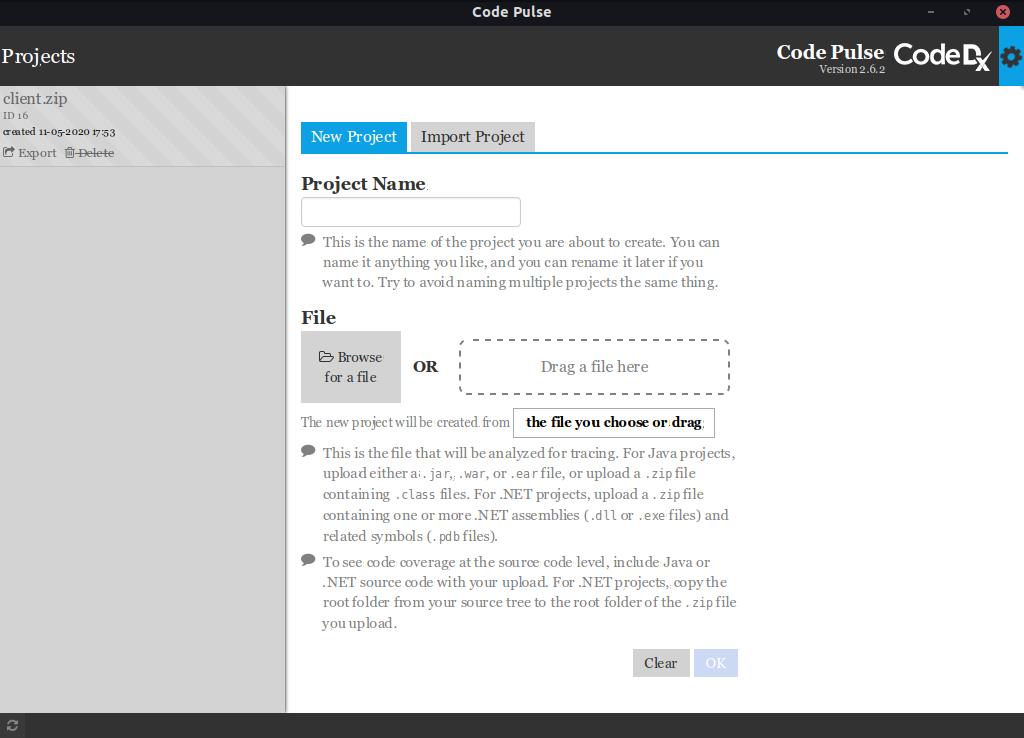
\includegraphics[scale = 0.31]{fig52.png}

  \caption{New Project}

\end{figure}
Aqui, como pode ser lido na própria janela, pode escolher-se o nome do projeto e indica como deve ser "entregue" o código a aplicação. Por exemplo, para o caso do Java deve ser entregue um Zip com o código compilado ou um Jar (melhor se estiverem contidas todas as depêndencias).

\par O programa irá procurar por CVE relacionados com as bibliotecas e/ou componentes usadas pelo programa e depois apresenta-los como é mostrado na figura seguinte:
\begin{figure}[H]

  \centering

  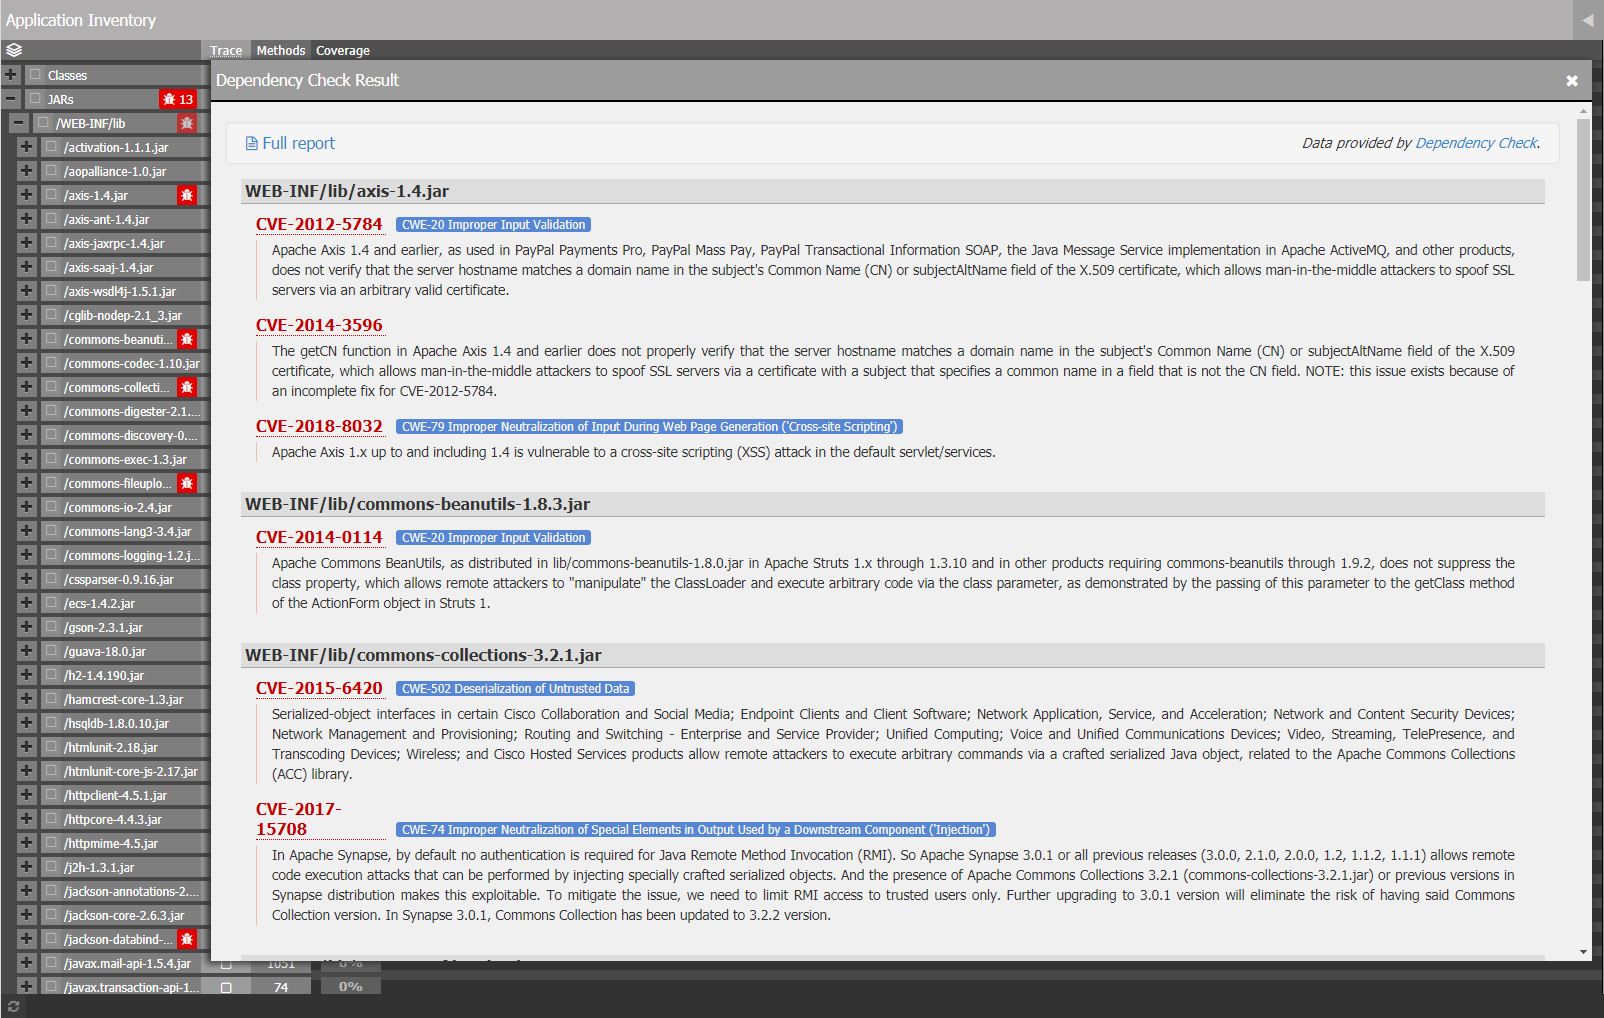
\includegraphics[scale = 0.21]{fig51.png}

  \caption{CVEs (Outro Programa)}

\end{figure}
A seguir, para começar os testes basta adicionar a flag que mostra na imagem seguinte a execução dos mesmos. Caso sejam, testes exclusivamente Black-Box adiciona-se ao programa a testar, caso seja a testes que o use o programa principal pode ser posto a flag nesses. Existem flags diferentes dependendo se estes são programas Java ou .Net. O programa ainda "permite" mudar a porta do agente, no entanto, não foi possível encontrar uma porta que este considera-se aberta para usar sem ser a que é considerada por defeito.
\begin{figure}[H]

  \centering

  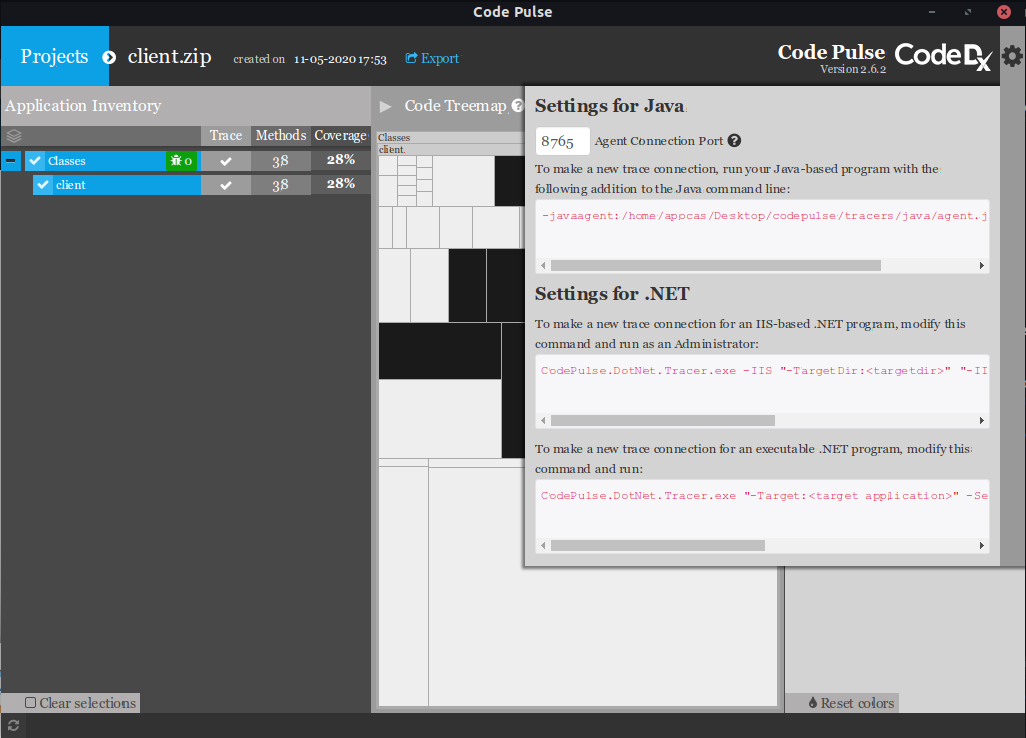
\includegraphics[scale = 0.31]{fig53.png}

  \caption{Flag de Tracing}

\end{figure}

\begin{figure}[H]

  \centering

  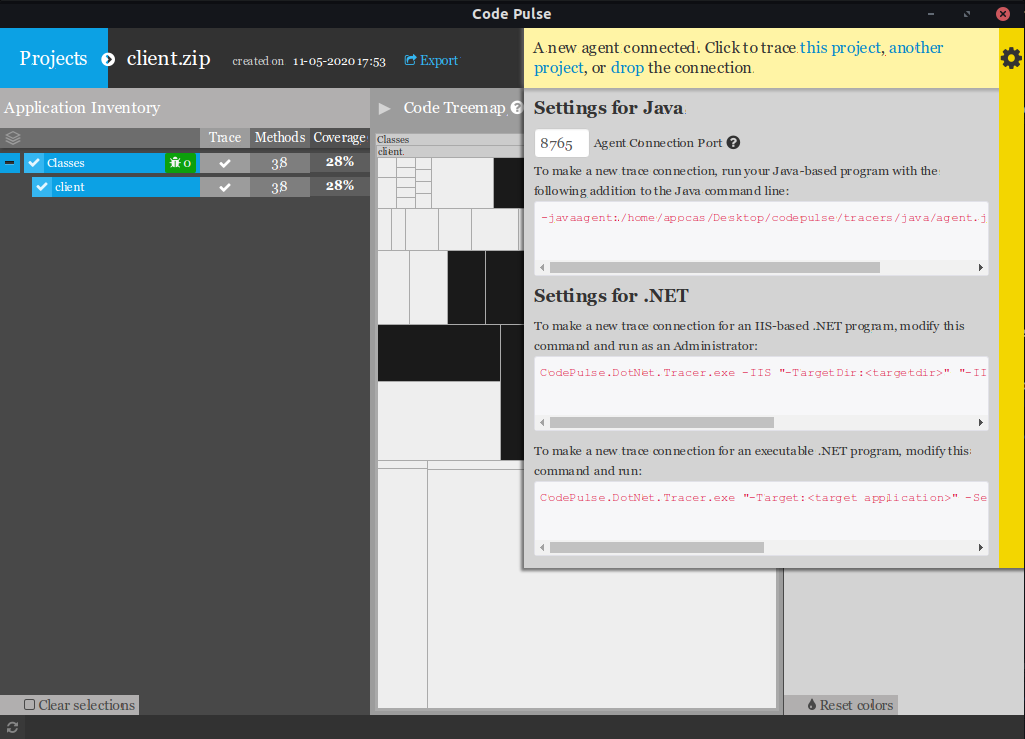
\includegraphics[scale = 0.31]{fig54.png}

  \caption{Linking Tracer}

\end{figure}
\par Ao iniciar o programa de teste/para teste com a flag devida irá aparecer um pop-up no Code Pulse na parte superior direita. Nesta fase pode fazer-se o link do tracer ao projeto, a outro projeto ou fazer drop da conexão do Tracer. A partir deste momento pode dar-se inicio aos testes. Obviamente, para começar deve escolher-se a primera opção.

\subsection{Funcionalidades}

\par A ferramenta para fazer o coverage apresenta o código de forma gráfica como se pode ver a na figura seguinte:

\begin{figure}[H]

  \centering

  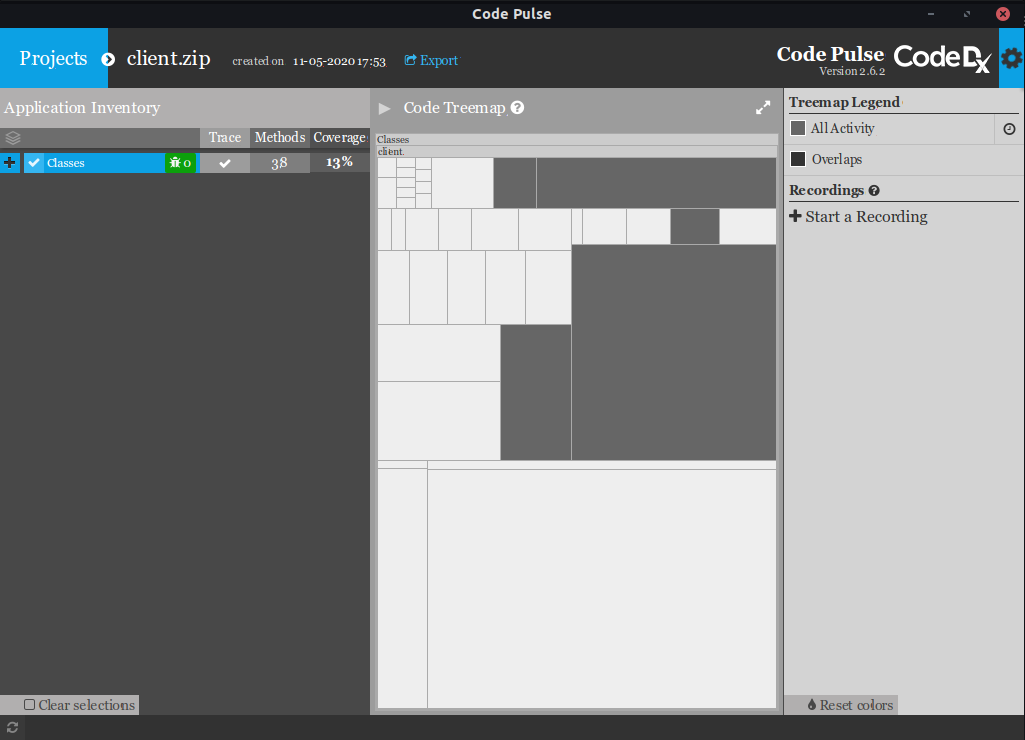
\includegraphics[scale = 0.31]{fig49.png}

  \caption{Code Pulse Interface}

\end{figure}

O TreeMap representa cada metodo em branco quando não foi usado seja por um método de teste ou por própria utilização do programa. Assim, pode realizar-se testes e ver qual porção foi "tocada".

\par Ainda pode-se definir cores para a atividade em geral, para os overlaps entre os diferentes recordings que, normalmente, seriam utilizados para separar diferentes test suites. E, assim, ter uma vista gráfica dos metodos que já foram testados e aqueles que precisam de maior número de testes.
\par Por exemplo, na imagem seguinte, vê-se a azul o resultado de um dos recordings, a verde outro, a cinzento metodos que foram cobertos mas em nenhum recording e finalmente a vermelho o overlap feito pelos dois recordings.
\par Os recordings pode ser selecinados, de forma a facilitar a comparação entre os mesmos e, consequentemente, os test suites associados.Ainda pode ser selecionados quais as componentes a fazer trace selecionado as checkbox a esquerda do programa. Ainda o programa apresenta o número de metodos de cada componente como a percentagem de coverage do mesmo. Adicionalmente, é possível, caso código seja fornecido ao Code Pulse, pode ser visto o próprio source code e analisar quais partes de certa função que foi utilizada. A figura seguinte ilustra esta funcionalidade2.

\begin{figure}[!htb]

  \centering

  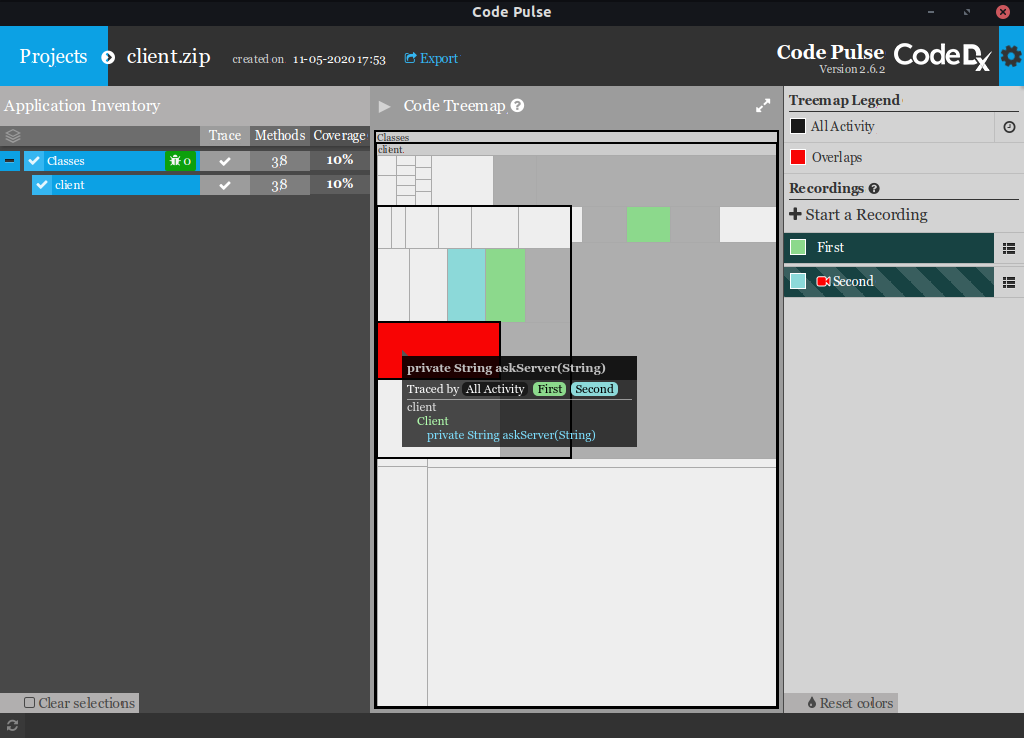
\includegraphics[width=\textwidth,height=50mm]{fig50.png}

  \caption{Recordings}

\end{figure}


\begin{figure}[H]

  \centering

  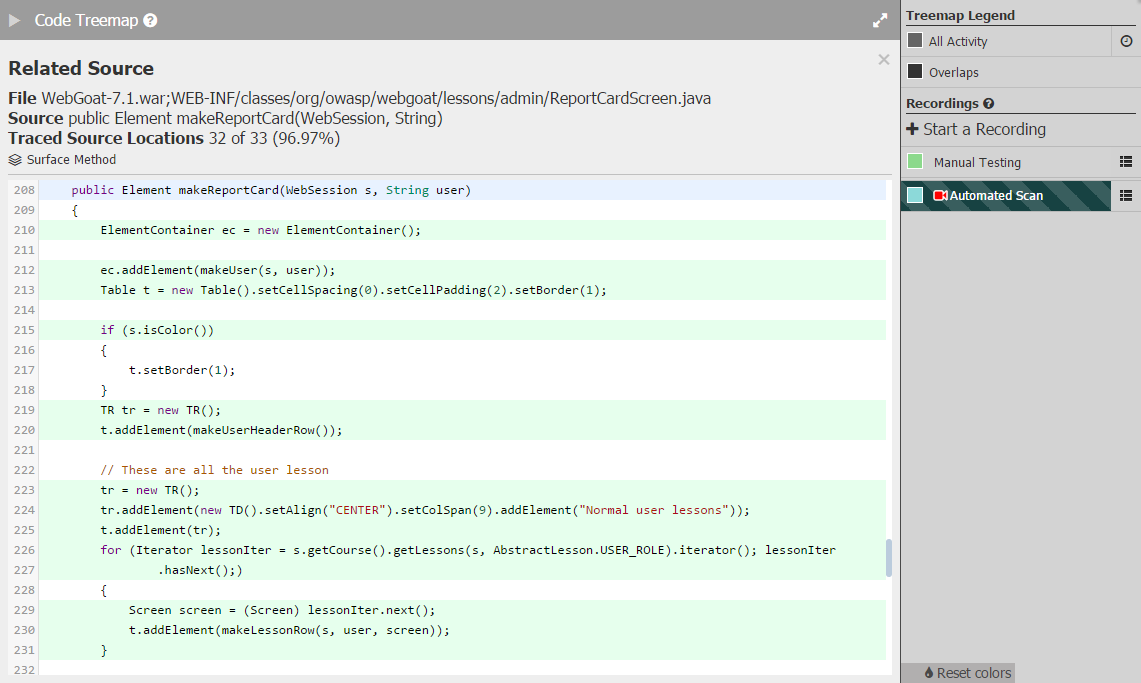
\includegraphics[scale = 0.31]{fig55.png}

  \caption{Source Code Viewer}

\end{figure}
\pagebreak
Note-se que para as aplicações Java, o Code Pulse considera a linha de código testada caso alguma porção de código contido nessa linha seja executado. No entanto, no caso de aplicações .NET é mais granular. Ainda, caso as classes JAVA ultrapassarem os 64KB não serão monitorizados.